\documentclass{article}
\usepackage{amsmath}
\usepackage{amssymb}
\usepackage[a4paper, top=25mm, bottom=25mm, left=25mm, right=25mm]{geometry}
\usepackage{pgfplots}
\usepackage{mathtools}
\usepgfplotslibrary{fillbetween}
\pgfplotsset{compat=1.18}

\begin{document}
\pagestyle{empty}
\large

\begin{center}
2017-2018 Summer \\MAT123-02 Final\\(13/08/2018)
\end{center}

\noindent 1. Let us consider the area $A$ of the region bounded by the curves $y=\mathrm{e}^x,\:y=x^2-1$ and the straight lines $x=-1,\:x=1$. Write an integral (but do not evaluate) corresponding to the area $A$ with respect to the $y$-axis.

\hfill

\noindent 2. Sketch the graph of

\[f(x)=\frac{4x}{x^2+1}.\]

\hfill

\noindent 3. Evaluate the following integrals.


\hfill

\noindent (a) $\displaystyle\int\frac{\tan x}{\sec^4x}\,dx$

\hfill

\hfill

\noindent (b) $\displaystyle\int\frac{\ln x}{x^3}\,dx$

\hfill

\hfill

\noindent (c) $\displaystyle\int\frac1{1+\sin x}\,dx$

\hfill

\hfill

\noindent (d) $\displaystyle\int\frac{x+7}{x^2\,(x+2)}\,dx$

\hfill

\hfill

\noindent 4. Use the Shell Method to determine the volume of the solid obtained by rotating the region bounded by $y=x^2-2x,\:y=x$ about the line $y=4$.

\hfill

\noindent 5. Find the area of the surface generated by rotating the curve $y=\mathrm{e}^x,\:0\leq x\leq1$ about the $x$-axis.

\hfill

\noindent 6. Use the Integral Test to investigate the convergence of the series $\displaystyle\sum_{k=0}^{\infty}k\mathrm{e}^{-k}$.

\hfill

\noindent 7. Find the Maclaurin series of the function $f(x)=\ln(1+x)$.

\hfill

\noindent 8. Find the interval of convergence of the power series $\displaystyle\sum_{n=1}^{\infty}\frac{(x-2)^n}{n\cdot 5^n}$.

\newpage

\begin{center}
2017-2018 Summer Final (13/08/2018) Solutions\\
(Last update: 30/08/2025 01:00)
\end{center}

\noindent 1.
\begin{center}
\begin{minipage}{0.33\textwidth}
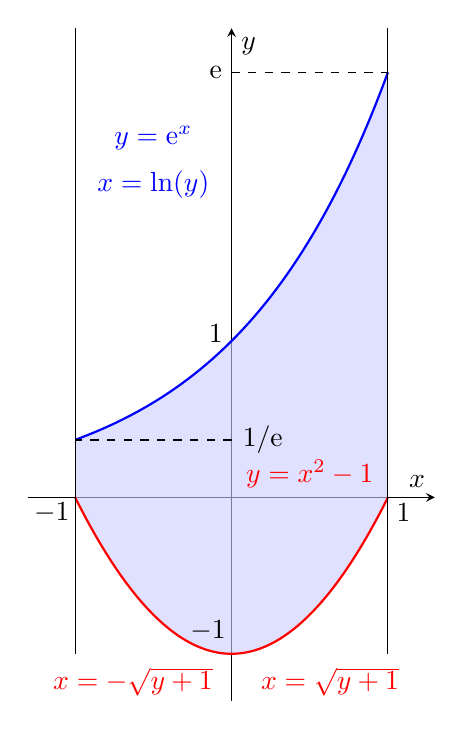
\begin{tikzpicture}
  \begin{axis}[
      axis lines=center,
      axis equal image,
      xlabel={$x$},
      ylabel={$y$},
      xtick=\empty, ytick=\empty,
      xmin=-1.3, xmax=1.3,
      ymin=-1.3, ymax=3,
      samples=200,
      scale=1.5,
      domain=-1:1,
    ]

    \addplot [thick, blue, name path=A, domain=-1:1] {e^x};
    \addplot [thick, red, name path=B] {x^2-1};
    \addplot [blue!20, fill opacity=0.6] fill between[of=A and B,soft clip={domain=-1:1}];
    \draw (-1,-1)--(-1,3); \draw (1,-1)--(1,3); \draw[dashed] (0,2.718)--(1,2.718); \draw[dashed] (0,0.367)--(-1,0.367);


    \node at (axis cs:-1.15,-0.1) {$-1$};
    \node at (axis cs:1.1,-0.1) {$1$};
    \node at (axis cs:-0.1,1.05) {$1$};
    \node at (axis cs:-0.15,-0.85) {$-1$};
    \node at (-0.1,2.718) {$\mathrm{e}$};
    \node at (0.2,0.367) {$1/\mathrm{e}$};
    \node[red] at (0.5,0.15) {$y=x^2-1$};
    \node[red] at (0.63,-1.18) {$x=\sqrt{y+1}$};
    \node[red] at (-0.63,-1.18) {$x=-\sqrt{y+1}$};

    \node[blue] at (-0.5,2.3) {$y=\mathrm{e}^x$};
    \node[blue] at (-0.5,2) {$x=\ln(y)$};

\end{axis}
\end{tikzpicture}
\end{minipage}
\begin{minipage}{0.62\textwidth}
\[\boxed{
\begin{array}{cl}
A=&\displaystyle\int_{-1}^0\left[\left(\sqrt{y+1}\right)-\left(-\sqrt{y+1}\right)\right]\,dy\\\\&+\displaystyle\int_0^{1/\mathrm{e}}\left[(1)-(-1)\right]\,dy+\displaystyle\int_{1/\mathrm{e}}^{\mathrm{e}}\left[(1)-\left(\ln y\right)\right]\,dy
\end{array}}\]
\end{minipage}
\end{center}

\hfill

\noindent 2. The function $f$ is defined where the denominator is not equal to zero. However, the denominator is always positive. Therefore, the domain of $f$ is $\mathbb{R}$.

\hfill

\noindent Let us find the limit at infinity and negative infinity.

\[\lim_{x\to\infty}\frac{4x}{x^2+1}=\lim_{x\to\infty}\frac{4}{x+\frac1x}=0\]

\hfill

\noindent Similarly, at negative infinity, the limit is zero. Therefore, the $x$-axis is a horizontal asymptote. There is no vertical asymptote.

\hfill

\noindent Take the first derivative and find the critical points. Apply the quotient rule.

\[y'=\frac d{dx}\left(\frac{4x}{x^2+1}\right)=\frac{4\cdot\left(x^2+1\right)-4x\cdot(2x)}{\left(x^2+1\right)^2}=\frac{-4x^2+4}{\left(x^2+1\right)^2}\]

\hfill

\noindent The critical points occur at $x=\pm1$. At these points, the first derivative is $0$.

\hfill

\noindent Take the second derivative. Apply the quotient rule again.

\[y''=\frac d{dx}\left(\frac{-4x^2+4}{\left(x^2+1\right)^2}\right)=\frac{\left(-8x\right)\cdot\left(x^2+1\right)^2-\left(-4x^2+4\right)\cdot2\left(x^2+1\right)\cdot(2x)}{\left(x^2+1\right)^4}=\frac{8x\left(x^2-3\right)}{\left(x^2+1\right)^3}\]

\hfill

\noindent The inflection points occur at $x=0$ and $x=\pm\sqrt3$. At these points, the direction of the curvature changes.

\hfill

\noindent Consider some values of the function. Eventually, set up a table and see what the graph looks like in certain intervals.

\[f\left(-\sqrt3\right)=-\sqrt3,\quad f(-1)=-2,\quad f(0)=0,\quad f(1)=2,\quad f\left(\sqrt3\right)=\sqrt3\]

\begin{center}
    \large
    \begin{tabular}{|c|cccccc|} 
    \hline
        $x$&$\left(-\infty,-\sqrt3\right)$&$\left(-\sqrt3,-1\right)$&$\left(-1,0\right)$&$\left(0,1\right)$&$\left(1,\sqrt3\right)$&$\left(\sqrt3,\infty\right)$\\
        \hline
        $y$&$\left(-\sqrt3,0\right)$&$\left(-2, -4\sqrt3\right)$&$(-2,0)$&$(0,2)$&$\left(\sqrt3,2\right)$&$\left(0,\sqrt3\right)$\\
        \hline
        $y'$ sign&-&-&+&+&-&-\\
        \hline
        $y''$ sign&-&+&+&-&-&+\\
        \hline
    \end{tabular}
\end{center}

\hfill

\begin{center}
\begin{tikzpicture}
  \begin{axis}[
    axis lines = center,
    xlabel = $x$, ylabel = $y$,
    domain=-13:13,
    samples=200,
    ymin=-2.2, ymax=2.2,
    xmin=-11, xmax=11,
    restrict y to domain=-5:5,
    enlargelimits=true,
    axis line style={->},
    xtick={-12,-8,-4,4,8,12}, ytick=\empty,
    scale=1.75,
    ]
    \addplot[blue, thick] {4*x/(x^2+1)};
    \draw[dashed](1.732,0)--(1.732,1.732) ;\draw[dashed](1,0)--(1,2); \draw[dashed](0,2)--(1,2); \draw[dashed](0, 1.732)--(1.732,1.732);
    \draw[dashed](-1.732,0)--(-1.732,-1.732) ;\draw[dashed](-1,0)--(-1,-2); \draw[dashed](0,-2)--(-1,-2); \draw[dashed](0, -1.732)--(-1.732,-1.732);
    
    \draw[dashed,red,thick] (-15,0.02)--(15,0.02);

    \node at (-0.75,0.15) {\small $-1$}; \node at (-2.2,0.15) {\small $-\sqrt3$};
    \node at (0.8,-0.15) {\small $1$}; \node at (1.85,-0.15) {\small $\sqrt3$};
    \node at (-0.5,2) {\small $2$}; \node at (-0.7,1.732) {\small $\sqrt3$};
    \node at (0.7,-2) {\small $-2$}; \node at (0.5,-1.732) {\small $-\sqrt3$};
    

  \end{axis}
\end{tikzpicture}
\end{center}

\noindent 3.

\hfill

\noindent (a) Try to rewrite in the form of $\sin x$ and $\cos x$.

\[\int\frac{\tan x}{\sec^4x}\,dx=\int\frac{\sin x}{\cos x}\cdot\cos^4x\,dx=\int\sin x\cdot\cos^3x\,dx=\int\sin x\cdot\left(1-\sin^2x\right)\cdot \cos x\,dx\]

\hfill

\noindent Let $u=\sin x$, then $du=\cos x\,dx$.

\begin{align*}\int\sin x\cdot\left(1-\sin^2x\right)\cdot\cos x\,dx&=\int u\left(1-u^2\right)\,du=\int\left(u-u^3\right)\,du=\frac{u^2}2-\frac{u^4}4+c\\\\&=\boxed{\frac{\sin^2x}2-\frac{\sin^4x}{4}+c,\quad c\in\mathbb{R}}\end{align*}

\newpage

\noindent (b) Use the method of integration by parts.

\[\left.\begin{array}{c}
u=\ln x\implies du=\dfrac1x\,dx\\[1em]
dv=\dfrac1{x^3}\,dx\implies v=-\dfrac1{2x^2}
\end{array}\right\}\rightarrow \int u\,dv=uv-\int v\,du\]

\[\int\frac{\ln x}{x^3}\,dx=-\frac{\ln x}{2x^2}-\int-\frac1{2x^3}\,dx=\boxed{-\frac{\ln x}{2x^2}-\frac1{4x^2}+c,\quad c\in\mathbb{R}}\]

\hfill

\noindent (c) Expand the expression by multiplying and dividing by the conjugate of the denominator.

\begin{align*}\int\frac1{1+\sin x}\,dx&=\int\frac{1-\sin x}{(1+\sin x)(1-\sin x)}\,dx=\int\frac{1-\sin x}{1-\sin^2x}\,dx=\int\frac{1-\sin x}{\cos^2x}\,dx\\\\&=\int\left(\sec^2x-\tan x\sec x\right)\,dx=\boxed{\tan x-\sec x+c,\quad c\in\mathbb{R}}\end{align*}

\hfill

\noindent (d) Use the method of partial fraction decomposition.

\[\int\frac{x+7}{x^2\,(x+2)}\,dx=\int\left(\frac{A}{x}+\frac{B}{x^2}+\frac{C}{x+2}\right)\,dx\]

\[\begin{array}{rc}
A(x)(x+2)+B(x+2)+C\left(x^2\right)&=x+7\\
x^2(A+C)+x(2A+B)+2B&=x+7
\end{array}\]

\hfill

\noindent Equate the coefficients of like terms.

\[\left.\begin{array}{c}
A+C=0\\
2A+B=1\\
2B=7
\end{array}\right\}\implies A=-\dfrac54, \quad B=\dfrac72,\quad C=\dfrac54\]

\hfill

\noindent Rewrite the integral by substituting the values into the unknowns.
\[\int\left(-\frac5{4x}+\frac{7}{2x^2}+\frac5{4(x+2)}\right)\,dx=\boxed{-\frac{5}4\ln\left|x\right|-\frac7{2x}+\frac54\ln\left|x+2\right|+c,\quad c\in\mathbb{R}}\]

\hfill

\noindent 4.
\begin{center}
\begin{minipage}{0.55\textwidth}
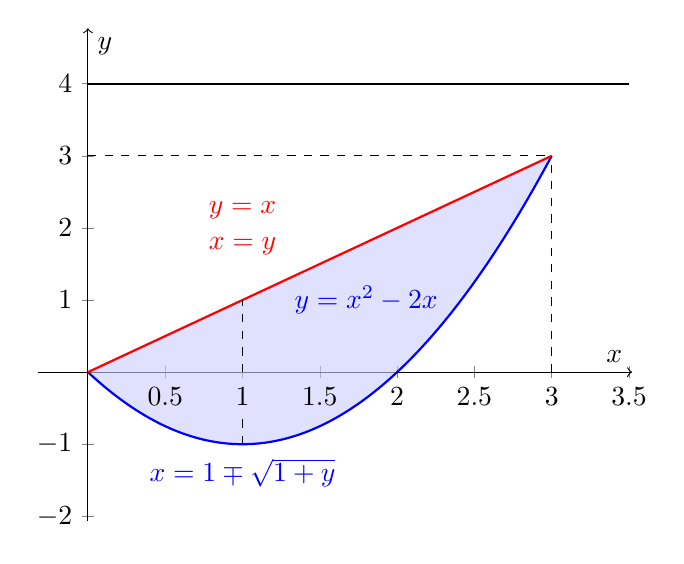
\begin{tikzpicture}
  \begin{axis}[
    axis lines = center,
    xlabel = $x$, ylabel = $y$,
    domain=0:3,
    samples=200,
    ymin=-1.5, ymax=4.2,
    xmin=0, xmax=3.2,
    enlargelimits=true,
    axis line style={->},
    scale=1.1,
    clip=true,
    ]
    \addplot[blue, thick, name path=A] {x^2-2*x};
    \addplot[red, thick, name path=B] {x};
    \addplot[blue!20, draw=none, opacity=0.6] fill between[of=A and B, soft clip={domain=0:3}];

    \draw[thick] (0,4)--(3.5,4);
    \draw[dashed] (1,-1)--(1,-0.6); \draw[dashed] (1,0)--(1,1);
    \draw[dashed] (3,0)--(3,3); \draw[dashed] (0,3)--(3,3);

    \node[red] at (1,2.25) {$y=x$};
    \node[red] at (1,1.75) {$x=y$};

    \node[blue] at (1.8,1) {$y=x^2-2x$};
    \node[blue] at (1,-1.4) {$x=1\mp\sqrt{1+y}$};

  \end{axis}
\end{tikzpicture}
\end{minipage}
\begin{minipage}{0.4\textwidth}
\[V=\int_D2\pi\cdot h(y)\cdot r(y)\,dy\]
\end{minipage}
\end{center}
\begin{align}V&=\int_{-1}^02\pi\left(4-y\right)\left[\left(1+\sqrt{1+y}\right)-\left(1-\sqrt{1+y}\right)\right]\,dy\nonumber\\\nonumber\\&\quad\:+\int_0^{3}2\pi(4-y)\left[\left(1+\sqrt{1+y}\right)-\left(y\right)\right]\,dy\nonumber\\\nonumber\\&=2\pi\int_{-1}^0(4-y)\left(2\sqrt{1+y}\right)\,dy+2\pi\int_0^3(4-y)\left(1+\sqrt{1+y}-y\right)\,dy\end{align}

\hfill

\noindent Evaluate the first integral in $(1)$. Let $u=1+y$, then $du=dy$.

\[y=-1\implies u=0,\qquad y=0\implies u=1\]
\begin{align*}\mathrm{I}_1&=\int_{-1}^0(4-y)\left(2\sqrt{1+y}\right)\,dy=2\int_0^1(5-u)\sqrt u\,du=10\int_0^1\sqrt u\,du-2\int_0^1u^{3/2}\,du\\\\&=\frac{20}3u^{3/2}-\frac45u^{5/2}\Bigg|_0^1=\frac{20}3-\frac45-0=\frac{88}{15}\end{align*}

\hfill

\noindent Evaluate the second integral in $(1)$. Let $u=1+y$, then $du=dy$.

\[y=0\implies u=1,\qquad y=3\implies u=4\]
\begin{align*}\mathrm{I}_2&=\int_0^3(4-y)\left(1+\sqrt{1+y}-y\right)\,dy=\int_1^4(5-u)\left(-u+2+\sqrt u\right)\,du\\\\&=\int_1^4\left(-7u+10+u^2+5\sqrt u-u^{3/2}\right)\,du=\left[-\frac{7u^2}2+10u+\frac{u^3}3+\frac{10}3u^{3/2}-\frac25u^{5/2}\right]_1^4\\\\&=\left[\left(-56+40+\frac{64}3+\frac{80}3-\frac{64}5\right)-\left(-\frac72+10+\frac13+\frac{10}3-\frac25\right)\right]=\frac{283}{30}\end{align*}

\hfill

\noindent Therefore, the result is

\[2\pi\left(\frac{88}{15}+\frac{283}{30}\right)=\boxed{\frac{153\pi}5}\]

\hfill

\noindent 5. If the function $y=f(x)\geq0$ is continuously differentiable on $[a,b]$, the area of the surface generated by revolving the graph of $y=f(x)$ about the $x$-axis is

\[S=\int_a^b2\pi y\sqrt{1+\left(\frac{dy}{dx}\right)^2}\,dx\]

\hfill

\noindent $\dfrac{dy}{dx}=\mathrm{e}^x$. Set $a=0,\:b=1,\:$ and then evaluate the integral.

\[S=\int_0^12\pi\mathrm{e}^x\sqrt{1+\left(\mathrm{e}^x\right)^2}\,dx\]

\hfill

\noindent Let $u=\mathrm{e}^x$, then $du=\mathrm{e}^x\,dx$.

\[x=0\implies u=\mathrm{e}^0=1,\qquad x=1\implies u=\mathrm{e}^1=\mathrm{e}\]

\[S=\int_0^12\pi\mathrm{e}^x\sqrt{1+\left(\mathrm{e}^x\right)^2}\,dx=2\pi\int_1^{\mathrm{e}}\sqrt{1+u^2}\,du\]

\hfill

\noindent We will now use a trigonometric substitution. Let $u=\tan t$ for $\displaystyle0<t<\frac\pi2$, then $du=\sec^2 t\,dt$.

\begin{align*}S&=2\pi\int_1^{\mathrm{e}}\sqrt{1+u^2}\,du=2\pi\int\sqrt{1+\tan^2t}\cdot\sec^2t\,dt=2\pi\int\sqrt{\sec^2t}\cdot\sec^2t\,dt\\\\&=2\pi\int\left|\sec t\right|\sec^2t\,dt=2\pi\int\sec^3t\,dt\qquad\left[\sec t>0\right]\end{align*}

\hfill

\noindent Find the antiderivative of $\sec^3t$ with the help of integration by parts.

\begin{align*}
    w=\sec t\,&\rightarrow\, dw = \sec t\tan t \,dt\\
    dz=\sec^2t\,dt\,&\rightarrow\, z = \tan t
\end{align*}
\begin{align*}
\int\sec^3t\,du&=\tan t\cdot\sec t-\int\tan^2 t\sec t\,dt=\tan t\cdot\sec t-\int\frac{1-\cos^2t}{\cos^3 t}\,dt\\\\&=\tan t\cdot\sec t-\int\sec^3t\,dt+\int\sec t\,dt 
\end{align*}

\hfill

\noindent Notice that the integral appears on the right side of the equation. Therefore,

\[\int\sec^3t\,dt=\frac12\cdot\tan t\cdot\sec t+\frac12\cdot\int\sec t\,dt\]

\hfill

\noindent The integral of $\sec t$ with respect to $t$ is

\[\int\sec t\,dt=\ln\left|\tan t+\sec t\right|+c_1,\quad c_1\in\mathbb{R}\]

\hfill

\noindent Recall $u=\tan t$.

\[u=\tan t\implies u^2=\tan^2t=\sec^2t-1\implies \sec t=\sqrt{u^2+1}\]

\begin{align*}S&=2\pi\cdot\frac12\left(\tan t\cdot\sec t+\ln\left|\tan t+\sec t\right|\right)+c=\pi\left[u\cdot\sqrt{u^2+1}+\ln\left|t+\sqrt{u^2+1}\right|\right]_1^{\mathrm{e}}\end{align*}

\begin{align*}S&=\pi\left[\left(\mathrm{e}\cdot\sqrt{\mathrm{e}^2+1}+\ln\left|\mathrm{e}+\sqrt{\mathrm{e}^2+1}\right|\right)-\left(\sqrt2+\ln\left|1+\sqrt2\right|\right)\right]\\\\&=\boxed{\pi\left[\mathrm{e}\cdot\sqrt{\mathrm{e}^2+1}-\sqrt2+\ln\left(\frac{\mathrm{e}+\sqrt{\mathrm{e}^2+1}}{1+\sqrt2}\right)\right]}\end{align*}

\hfill

\noindent 6. Let the corresponding function be $f(x)=x\mathrm{e}^{-x}$. $f$ is continuous for $x\geq0$. $f$ is positive for $x\geq0$ because $x\geq 0$ and $\mathrm{e}^{-x}$ is positive everywhere. The function is also decreasing for $x\geq1$. Verify this behavior by taking the first derivative of $f$. Apply the product rule.

\[f'(x)=1\cdot\mathrm{e}^{-x}-x\mathrm{e}^{-x}=(1-x)\mathrm{e}^{-x}\]

\hfill

\noindent $f'(x)>0$ for $x\geq1$. The Integral Test states that all the conditions must be satisfied for and after a specific value, for instance $x=1$. Therefore, set the lower bound $x=1$ and evaluate the integral. We will exclusively evaluate the first term of the sequence thereafter.

\[\int_1^{\infty}x\mathrm{e}^{-x}\,dx\]

\hfill

\noindent Apply integration by parts and then evaluate the improper integrals by taking the limit.

\[\left.\begin{array}{c}
u=x\implies du=dv\\[1em]
dv=\mathrm{e}^{-x}\,dx\implies v=-\mathrm{e}^{-x}
\end{array}\right\}\rightarrow \int u\,dv=uv-\int v\,du\]

\begin{align*}\int_1^{\infty}x\mathrm{e}^{-x}\,dx&=\lim_{R\to\infty}\left[-x\mathrm{e}^{-x}\right]_1^R-\lim_{P\to\infty}\int_1^P-\mathrm{e}^{-x}\,dx=\lim_{R\to\infty}\left[-x\mathrm{e}^{-x}\right]_1^R-\lim_{P\to\infty}\mathrm{e}^{-x}\bigg|_1^P\\\\&=\lim_{R\to\infty}\left(-R\mathrm{e}^{-R}+\mathrm{e}^{-1}\right)-\lim_{P\to\infty}\left(\mathrm{e}^{-P}-\mathrm{e}^{-1}\right)=\lim_{R\to\infty}\left(-R\mathrm{e}^{-R}\right)+2\mathrm{e}^{-1}\end{align*}

\hfill

\noindent To evaluate the limit, we assume that $-R\mathrm{e}^{-R}$ is a function of $R$. After that, put the expression in a form that we can apply L'Hôpital's rule in order to eliminate the form $\infty/\infty$.

\[\lim_{R\to\infty}\left(-R\mathrm{e}^{-R}\right)=\lim_{R\to\infty}\frac{-R}{\frac1{\mathrm{e}^{-R}}}\overset{\text{L'H.}}{=}\lim_{R\to\infty}\frac1{\frac{1}{\mathrm{e}^{-2R}}\cdot\left(-\mathrm{e}^{-R}\right)}=\lim_{R\to\infty}\left(-\mathrm{e}^{-R}\right)=0\]

\hfill

\noindent Since the integral converges to $2\mathrm{e}^{-1}$, the series $\displaystyle\sum_{k=1}^{\infty}k\mathrm{e}^{-k}$ also converges. The first term of the series in the original question is $0\cdot\mathrm{e}^0=0$. The sum of a convergent series and a finite number is still finite. Therefore, the sum $\displaystyle\sum_{k=0}^{\infty}k\mathrm{e}^{-k}$ converges.

\newpage

\noindent 7. The Maclaurin series of $f$ is as follows.

\[\sum_{k=0}^{\infty}\frac{f^{(k)}(0)}{k!}x^k\]

\hfill

\noindent Find $f(0),\:f'(0),\:f''(0),\:f'''(0),f^{(4)}(0)$ to look for the pattern.

\[f'(x)=\frac1{1+x},\quad f''(x)=-\frac1{(1+x)^2},\quad f'''(x)=\frac2{(1+x)^3}\quad f^{(4)}(x)=-\frac6{(1+x)^4} \]

\[f(0)=0,\quad f'(0)=1,\quad f''(0)=-1,\quad f'''(0)=2,\quad f^{(4)}(0)=-6\]

\hfill

\noindent This is an alternating sequence where the coefficient of each term is the factorial of the subsequent number starting from $0$ except for $k=0$, that is, the first term of the series. At $k=0$, the first term is $0$. So,

\[f^{k}(0)=\left\{\begin{array}{ll}(-1)^{k-1}\cdot (k-1)!,&\text{if}\: k>0\\0,& \text{if}\:k=0\end{array}\right.\]
\begin{align*}\sum_{k=0}^{\infty}\frac{f^{(k)}(0)}{k!}x^k&=0+\sum_{k=1}^{\infty}\frac{f^{(k)}(0)}{k!}x^k=\sum_{k=1}^{\infty}\frac{(-1)^{k-1}\cdot(k-1)!}{k\cdot(k-1)!}x^k\\\\&=\boxed{\sum_{k=1}^{\infty}\frac{(-1)^{k-1}\cdot x^k}{k}=x-\frac{x^2}2+\frac{x^3}3-\frac{x^4}4+...}\end{align*}

\hfill

\noindent 8. Apply the Ratio Test for absolute convergence, and apply other tests at the endpoints.

\[\lim_{n\to\infty}\left|\frac{(x-2)^{n+1}}{(n+1)\cdot(5)^{n+1}}\cdot\frac{n\cdot5^n}{(x-2)^n}\right|=\lim_{n\to\infty}\left|\frac{\left(x-2\right)\cdot n}{(n+1)\cdot5}\right|=\frac{|x-2|}5\cdot\lim_{n\to\infty}\left|\frac{n}{n+1}\right|=\frac{|x-2|}5\]
\[\frac{|x-2|}5<1\implies |x-2|<5\implies -5<x-2<5\implies -3<x<7 \quad (\text{convergent})\]

\hfill

\noindent Now, take a look at the endpoints.

\[x=-3\implies \sum_{n=1}^{\infty}\frac{(-5)^n}{n\cdot5^n}=\sum_{n=1}^{\infty}\frac{(-1)^n}n\]

\hfill

\noindent This is an alternating series. The non-alternating part, which is $\frac1n$, is nonincreasing for $n\geq1$ and it is positive. The limit at infinity is $0$. By Leibniz's Alternating Series Test, the series converges. Try $x=7$.

\[x=7\implies\sum_{n=1}^{\infty}\frac{(5)^n}{n\cdot5^n}=\sum_{n=1}^{\infty}\frac1n\]

\hfill

\noindent This is a $p$-series with $p=1$, for which the series diverges by the $p$-series Test.

\hfill

\noindent The convergence set for the power series is $\boxed{[-3,7)}$.

\end{document}